\section{寄存器描述}
\regover{
{\hyperref[psram-psram-configure]{psram\_configure}}&
\\
\hline
{\hyperref[psram-psram-manual-control]{psram\_manual\_control}}&
\\
\hline
{\hyperref[psram-fifo-thres-control]{fifo\_thres\_control}}&
\\
\hline
{\hyperref[psram-psram-manual-control2]{psram\_manual\_control2}}&
\\
\hline
{\hyperref[psram-winbond-psram-configure]{winbond\_psram\_configure}}&
\\
\hline
{\hyperref[psram-winbond-psram-status]{winbond\_psram\_status}}&
\\
\hline
{\hyperref[psram-winbond-psram-configure2]{winbond\_psram\_configure2}}&
\\
\hline
{\hyperref[psram-apmemory-psram-configure]{apmemory\_psram\_configure}}&
\\
\hline
{\hyperref[psram-apmemory-psram-status]{apmemory\_psram\_status}}&
\\
\hline
{\hyperref[psram-psram-manual-control3]{psram\_manual\_control3}}&
\\
\hline
{\hyperref[psram-psram-intf-delay-ctrl0]{psram\_intf\_delay\_ctrl0}}&
\\
\hline
{\hyperref[psram-psram-intf-delay-ctrl1]{psram\_intf\_delay\_ctrl1}}&
\\
\hline
{\hyperref[psram-psram-intf-delay-ctrl2]{psram\_intf\_delay\_ctrl2}}&
\\
\hline
{\hyperref[psram-psram-intf-delay-ctrl3]{psram\_intf\_delay\_ctrl3}}&
\\
\hline
{\hyperref[psram-psram-intf-delay-ctrl4]{psram\_intf\_delay\_ctrl4}}&
\\
\hline
{\hyperref[psram-psram-intf-delay-ctrl5]{psram\_intf\_delay\_ctrl5}}&
\\
\hline
{\hyperref[psram-psram-intf-delay-ctrl6]{psram\_intf\_delay\_ctrl6}}&
\\
\hline
{\hyperref[psram-psram-intf-delay-ctrlB]{psram\_intf\_delay\_ctrlB}}&
\\
\hline
{\hyperref[psram-psram-dbg-sel]{psram\_dbg\_sel}}&
\\
\hline
{\hyperref[psram-psram-dummy-reg]{psram\_dummy\_reg}}&
\\
\hline
{\hyperref[psram-psram-timeout-reg]{psram\_timeout\_reg}}&
\\
\hline
{\hyperref[psram-psram-rough-delay-ctrl0]{psram\_rough\_delay\_ctrl0}}&
\\
\hline
{\hyperref[psram-psram-rough-delay-ctrl1]{psram\_rough\_delay\_ctrl1}}&
\\
\hline
{\hyperref[psram-psram-rough-delay-ctrl2]{psram\_rough\_delay\_ctrl2}}&
\\
\hline
{\hyperref[psram-psram-rough-delay-ctrl3]{psram\_rough\_delay\_ctrl3}}&
\\
\hline
{\hyperref[psram-psram-rough-delay-ctrl4]{psram\_rough\_delay\_ctrl4}}&
\\
\hline
{\hyperref[psram-psram-rough-delay-ctrl5]{psram\_rough\_delay\_ctrl5}}&
\\
\hline
{\hyperref[psram-psram-rough-delay-ctrl6]{psram\_rough\_delay\_ctrl6}}&
\\
\hline
{\hyperref[psram-psram-rough-delay-ctrl7]{psram\_rough\_delay\_ctrl7}}&
\\
\hline
{\hyperref[psram-psram-rough-delay-ctrl8]{psram\_rough\_delay\_ctrl8}}&
\\
\hline
{\hyperref[psram-psram-rough-delay-ctrl9]{psram\_rough\_delay\_ctrl9}}&
\\
\hline
{\hyperref[psram-psram-rough-delay-ctrlA]{psram\_rough\_delay\_ctrlA}}&
\\
\hline
{\hyperref[psram-psram-rough-delay-ctrlB]{psram\_rough\_delay\_ctrlB}}&
\\
\hline
}

\subsection{psram\_configure}
\label{psram-psram-configure}
地址:0x4001a000
 \begin{figure}[H]
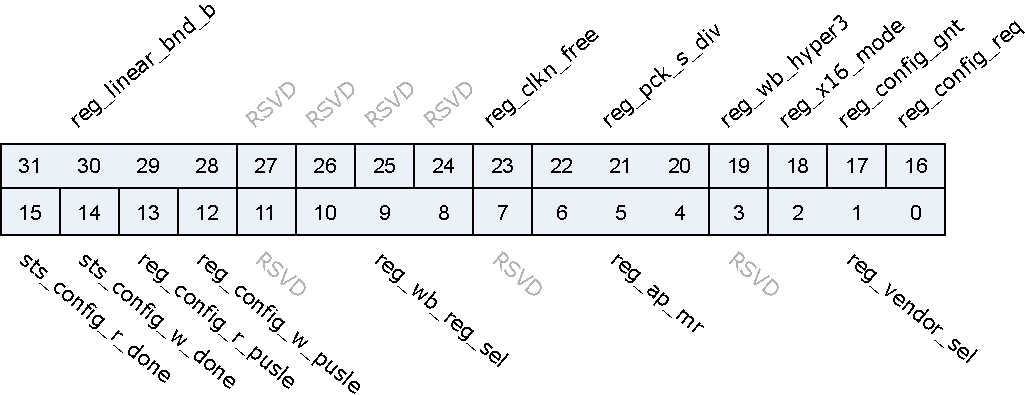
\includegraphics{psram_psram_configure.pdf}
\end{figure}

\regdes{31:28&reg\_linear\_bnd\_b&r/w&4'd10&Linear burst boundary shift bit\\\hline
27:24&RSVD& & & \\\hline
23&reg\_clkn\_free&r/w&1'b1&Clock\# free run\\\hline
22:20&reg\_pck\_s\_div&r/w&3'd0&EMI AXI bus clock division from psram\_ck\\\hline
19&reg\_wb\_hyper3&r/w&1'b0&Winbond Hyper3 bus\\\hline
18&reg\_x16\_mode&r/w&1'b0&16-bit pSRAM mode enable\\\hline
17&reg\_config\_gnt&r&1'b0&pSRAM register configure grant\\\hline
16&reg\_config\_req&r/w&1'b0&pSRAM register configure request\\\hline
15&sts\_config\_r\_done&r&1'b1&pSRAM register read done\\\hline
14&sts\_config\_w\_done&r&1'b1&pSRAM register write done\\\hline
13&reg\_config\_r\_pusle&w1p&1'b0&pSRAM configuration read enable\\\hline
12&reg\_config\_w\_pusle&w1p&1'b0&pSRAM configuration write enable\\\hline
11&RSVD& & & \\\hline
10:8&reg\_wb\_reg\_sel&r/w&2'd0&Winbond pSRAM Register R/W selection \par 3'd0 - ID0 / 3'd1 - ID1 \par 3'd2 - CR0 / 3'd3 - CR1 /3'd4 - CR2 \par 3'd5 - CR3 / 3'd6 - CR4
\\\hline
7&RSVD& & & \\\hline
6:4&reg\_ap\_mr&r/w&3'd0&APMemory pSRAM Mode Register R/W selection \par 3'd0=MA0 / 3'd1=MA1 / \par 3'd2=MA2 / 3'd3=MA3 / \par 3'd4=MA4 / 3'd6=MA6 / \par 3'd7=MA8
\\\hline
3&RSVD& & & \\\hline
2:0&reg\_vendor\_sel&r/w&3'b010&pSRAM vendor selection \par [0] - Winbond \par [1] - APM\_XCELLA \par [2] - APM\_HYPER
\\\hline

}
\subsection{psram\_manual\_control}
\label{psram-psram-manual-control}
地址:0x4001a004
 \begin{figure}[H]
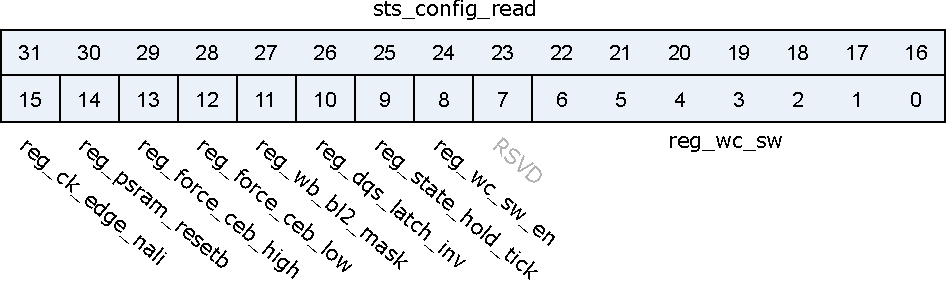
\includegraphics{psram_psram_manual_control.pdf}
\end{figure}

\regdes{31:16&sts\_config\_read&r&16'd0&full data from psram register read\\\hline
15&reg\_ck\_edge\_nali&r/w&1'b0&pSRAM clock 2x1x edge alignment \par 1'b0 - 2x/1x edge align \par 1'b1 - 2x/1x edge stagger
\\\hline
14&reg\_psram\_resetb&r/w&1'b1&pSRAM reset pin control\\\hline
13&reg\_force\_ceb\_high&r/w&1'b0&Force pSRAM ceb pin high\\\hline
12&reg\_force\_ceb\_low&r/w&1'b0&Force pSRAM ceb pin low(higher priority)\\\hline
11&reg\_wb\_bl2\_mask&r/w&1'b1&pSRAM Winbond burst length bit2 mask\\\hline
10&reg\_dqs\_latch\_inv&r/w&1'b0&pSRAM DQS latch invert\\\hline
9&reg\_state\_hold\_tick&r/w&1'b0&pSRAM hold state clock tick\\\hline
8&reg\_wc\_sw\_en&r/w&1'd0&pSRAM wait cycle sw mode enable\\\hline
7&RSVD& & & \\\hline
6:0&reg\_wc\_sw&r/w&7'd0&pSRAM sw mode wait cycle value\\\hline

}
\subsection{fifo\_thres\_control}
\label{psram-fifo-thres-control}
地址:0x4001a008
 \begin{figure}[H]
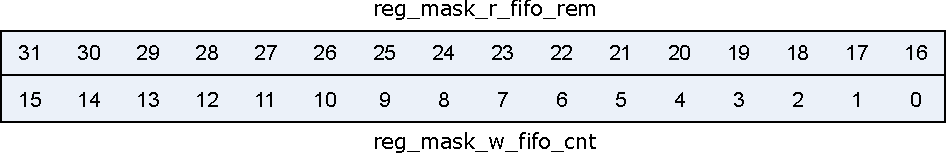
\includegraphics{psram_fifo_thres_control.pdf}
\end{figure}

\regdes{31:16&reg\_mask\_r\_fifo\_rem&r/w&16'h0&Read data fifo remain cnt threshold\\\hline
15:0&reg\_mask\_w\_fifo\_cnt&r/w&16'h0&Write data fifo data cnt threshold\\\hline

}
\subsection{psram\_manual\_control2}
\label{psram-psram-manual-control2}
地址:0x4001a00c
 \begin{figure}[H]
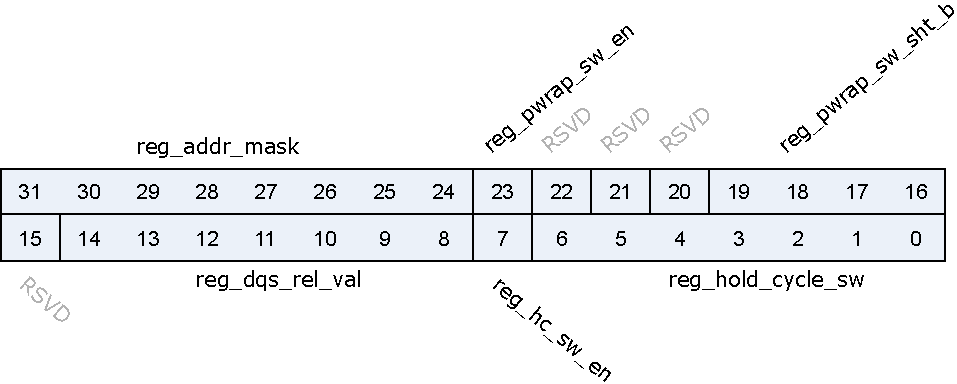
\includegraphics{psram_psram_manual_control2.pdf}
\end{figure}

\regdes{31:24&reg\_addr\_mask&r/w&8'h1f&pSRAM memory address mask for [27:20]\\\hline
23&reg\_pwrap\_sw\_en&r/w&1'd0&pSRAM WRAP sw setting enable (default off) \par Note - When using APS256XXN and setting burst length to 2'b11, it is necessary to set this register to 1
\\\hline
22:20&RSVD& & & \\\hline
19:16&reg\_pwrap\_sw\_sht\_b&r/w&4'd8&pSRAM WRAP sw setting value \par Note - When using APS256XXN and setting burst length to 2'b11, it is necessary  to set this register to 4'd11
\\\hline
15&RSVD& & & \\\hline
14:8&reg\_dqs\_rel\_val&r/w&7'h20&pSRAM dqs\_oen release counter value\\\hline
7&reg\_hc\_sw\_en&r/w&1'd0&pSRAM hold cycle sw mode enable\\\hline
6:0&reg\_hold\_cycle\_sw&r/w&7'd8&pSRAM sw mode hold cycle value\\\hline

}
\subsection{winbond\_psram\_configure}
\label{psram-winbond-psram-configure}
地址:0x4001a010
 \begin{figure}[H]
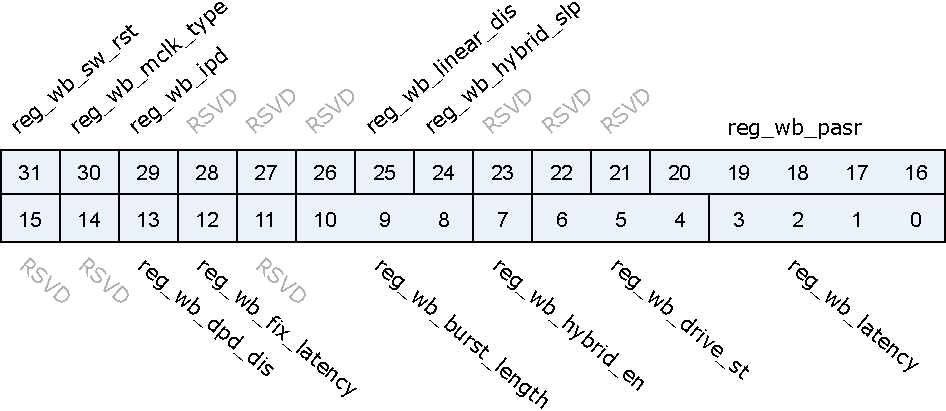
\includegraphics{psram_winbond_psram_configure.pdf}
\end{figure}

\regdes{31&reg\_wb\_sw\_rst&r/w&1'b0&Winbond pSRAM CR1 - Software Reset \par Trigger software reset (if device supprts)
\\\hline
30&reg\_wb\_mclk\_type&r/w&1'b1&Winbond pSRAM CR1 - Master Clock Type \par 0 - Differential CK\#, CK \par 1 - Single Ended
\\\hline
29&reg\_wb\_ipd&r/w&1'b0&Winbond pSRAM CR1 - Input Power Down \par 0 - Normal \par 1 - Enter Input Power Down Mode
\\\hline
28:26&RSVD& & & \\\hline
25&reg\_wb\_linear\_dis&r/w&1'b0&Winbond pSRAM linear burst disable\\\hline
24&reg\_wb\_hybrid\_slp&r/w&1'b0&Winbond pSRAM CR1 - Hybrid Sleep Mode configuration \par 1'b0 - Normal operation \par 1'b1 - Enter Hybrid Sleep Mode
\\\hline
23:21&RSVD& & & \\\hline
20:16&reg\_wb\_pasr&r/w&5'd0&Winbond pSRAM CR1 - Partial Array Refresh + Distributed Refresh Interval \par -------------------------------------------------------------------------------------------------------------------------------- \par For pSRAM >4MB [20:18] ; For pSRAM=4MB [18:16] \par 3'b000 - Full array / 3'b001 - Bottom 1/2 array / 3'b010 - Bottom 1/4 array / 3'b011 - Bottom 1/8 array \par 3'b100 - RSVD / 3'b101 - Top 1/2 array / 3'b110 - Top 1/4 array / 3'b111 - Top 1/8 array \par -------------------------------------------------------------------------------------------------------------------------------- \par For pSRAM >4MB [17:16]  \par 2'b10 - 1us / 2'b01 - 4is
\\\hline
15:14&RSVD& & & \\\hline
13&reg\_wb\_dpd\_dis&r/w&1'b1&Winbond pSRAM CR0 - Deep Power-Down Disable configuration \par 1'b0 - Deep sleep enable \par 1'b1 - Normal operation
\\\hline
12&reg\_wb\_fix\_latency&r/w&1'b1&Winbond pSRAM CR1 - Fix Latency configuration \par 1'b0 - Variable \par 1'b1 - Fixed
\\\hline
11&RSVD& & & \\\hline
10:8&reg\_wb\_burst\_length&r/w&3'd7&Winbond pSRAM CR0 - Burst Length configuration \par ------------------------------------------ \par For Non-Hyper Bus3 \par 3'b100 - 128 Byte \par 3'b101 - 64 Byte \par 3'b110 - 16 Byte \par 3'b111 - 32 Byte \par ------------------------------------------ \par For Hyper Bus3 \par 3'b100 - 128 Beat \par 3'b101 - 64 Beat \par 3'b110 - 16 Beat \par 3'b111 - 32 Beat \par 3'b011 - 512 Beat
\\\hline
7&reg\_wb\_hybrid\_en&r/w&1'b1&Winbond pSRAM CR0 - Hybrid Burst Enable \par 1'b0 - hybrid burst  \par 1'b1 - wrapped burst
\\\hline
6:4&reg\_wb\_drive\_st&r/w&3'd0&Winbond pSRAM CR0 - Drive Strength configuration \par for 4MB pSRAM \par 3'b00 - 50Ω / 3'b01 - 35Ω / 3'b10 - 100Ω / 3'b11 - 200Ω \par For 8MB pSRAM \par 3'b000 - 34Ω / 3'b001 - 115Ω / 3'b010 - 67Ω / 3'b011 - 46Ω \par 3'b100 - 34Ω / 3'b101 - 27Ω / 3'b110 - 22Ω / 3'b111 - 19Ω
\\\hline
3:0&reg\_wb\_latency&r/w&4'd2&Winbond pSRAM CR0 - Latency Counter configuration \par -------------------------------------------------------------- \par For Non-Hyper Bus3 \par 4'b0000 - Latency = 5 / Max freq. = 133 MHz \par 4'b0001 - Latency = 6 / Max freq. = 166 MHz \par 4'b0010 - Latency = 7 / Max freq. = 200 MHz \par 4'b1110 - Latency = 3 / Max freq. = 83 MHz \par 4'b1111 - Latency = 4 / Max freq. = 100 MHz \par Others - RSVD \par -------------------------------------------------------------- \par For Hyper Bus3 \par 4'b0111 - Latency = 14 / Max freq. = 400 MHz \par 4'b1001 - Latency = 19 / Max freq. = 533 MHz
\\\hline

}
\subsection{winbond\_psram\_status}
\label{psram-winbond-psram-status}
地址:0x4001a014
 \begin{figure}[H]
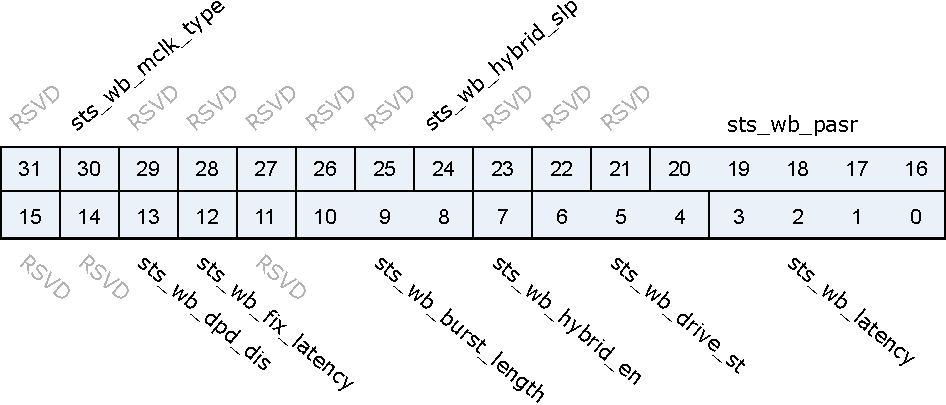
\includegraphics{psram_winbond_psram_status.pdf}
\end{figure}

\regdes{31&RSVD& & & \\\hline
30&sts\_wb\_mclk\_type&r&1'b1&Winbond pSRAM CR1 - Master Clock Type \par 0 - Differential CK\#, CK \par 1 - Single Ended
\\\hline
29:25&RSVD& & & \\\hline
24&sts\_wb\_hybrid\_slp&r&1'b0&Winbond pSRAM CR1 - Hybrid Sleep Mode configuration
 \par 1'b0 - Normal operation
 \par 1'b1 - Enter Hybrid Sleep Mode
\\\hline
23:21&RSVD& & & \\\hline
20:16&sts\_wb\_pasr&r&5'd0&Winbond pSRAM CR1 - Partial Array Refresh + Distributed Refresh Interval \par For pSRAM >4MB [20:18] ; For pSRAM=4MB [18:16] \par 3'b000 - Full array / 3'b001 - Bottom 1/2 array / 3'b010 - Bottom 1/4 array / 3'b011 - Bottom 1/8 array \par 3'b100 - RSVD / 3'b101 - Top 1/2 array / 3'b110 - Top 1/4 array / 3'b111 - Top 1/8 array \par For pSRAM >4MB [17:16]  \par 2'b10 - 1us / 2'b01 - 4is
\\\hline
15:14&RSVD& & & \\\hline
13&sts\_wb\_dpd\_dis&r&1'b1&Winbond pSRAM CR0 - Deep Power-Down Disable configuration
 \par 1'b0 - Deep sleep enable
 \par 1'b1 - Normal operation
\\\hline
12&sts\_wb\_fix\_latency&r&1'b1&Winbond pSRAM CR0 - Fix Latency configuration
 \par 1'b0 - Variable
 \par 1'b1 - Fixed
\\\hline
11&RSVD& & & \\\hline
10:8&sts\_wb\_burst\_length&r&3'd3&Winbond pSRAM CR0 - Burst Length configuration \par ------------------------------------------ \par For Non-Hyper Bus3 \par 3'b100 - 128 Byte \par 3'b101 - 64 Byte \par 3'b110 - 16 Byte \par 3'b111 - 32 Byte \par ------------------------------------------ \par For Hyper Bus3 \par 3'b100 - 128 Beat \par 3'b101 - 64 Beat \par 3'b110 - 16 Beat \par 3'b111 - 32 Beat \par 3'b011 - 512 Beat
\\\hline
7&sts\_wb\_hybrid\_en&r&1'b1&Winbond pSRAM CR0 - Hybrid Burst Enable \par 1'b0 - hybrid burst  \par 1'b1 - wrapped burst
\\\hline
6:4&sts\_wb\_drive\_st&r&2'd0&Winbond pSRAM CR0 - Drive Strength configuration \par for 4MB pSRAM \par 3'b00 - 50Ω / 3'b01 - 35Ω / 3'b10 - 100Ω / 3'b11 - 200Ω \par For 8MB pSRAM \par 3'b000 - 34Ω / 3'b001 - 115Ω / 3'b010 - 67Ω / 3'b011 - 46Ω  \par 3'b100 - 34Ω / 3'b101 - 27Ω / 3'b110 - 22Ω / 3'b111 - 19Ω
\\\hline
3:0&sts\_wb\_latency&r&4'd2&Winbond pSRAM CR0 - Latency Counter configuration \par -------------------------------------------------------------- \par For Non-HS mode :  \par 4'b0000 - Latency = 5 / Max freq. = 133 MHz \par 4'b0001 - Latency = 6 / Max freq. = 166 MHz \par 4'b0010 - Latency = 7 / Max freq. = 200 MHz \par 4'b1110 - Latency = 3 / Max freq. = 83 MHz \par 4'b1111 - Latency = 4 / Max freq. = 100 MHz \par Others - RSVD \par -------------------------------------------------------------- \par For HS mode \par 4'b0111 - Latency = 14 / Max freq. = 400 MHz \par 4'b1001 - Latency = 19 / Max freq. = 533 MHz
\\\hline

}
\subsection{winbond\_psram\_configure2}
\label{psram-winbond-psram-configure2}
地址:0x4001a018
 \begin{figure}[H]
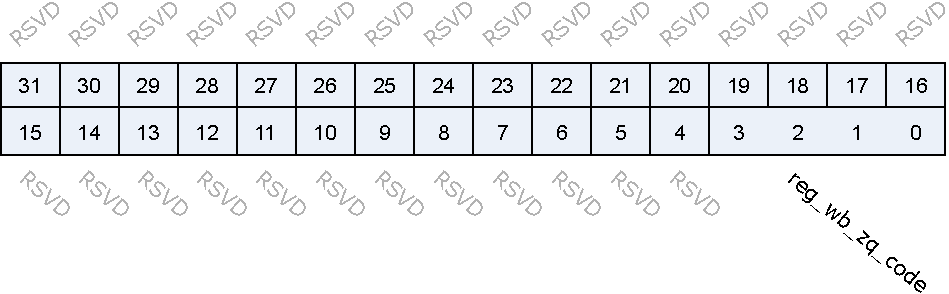
\includegraphics{psram_winbond_psram_configure2.pdf}
\end{figure}

\regdes{31:4&RSVD& & & \\\hline
3:0&reg\_wb\_zq\_code&r/w&4'd0&Winbond pSRAM CR2 - ZQ Calibration Code \par 4'b1111 : ZQ Calibration command \par 4'b0011 : ZQ Reset
\\\hline

}
\subsection{apmemory\_psram\_configure}
\label{psram-apmemory-psram-configure}
地址:0x4001a020
 \begin{figure}[H]
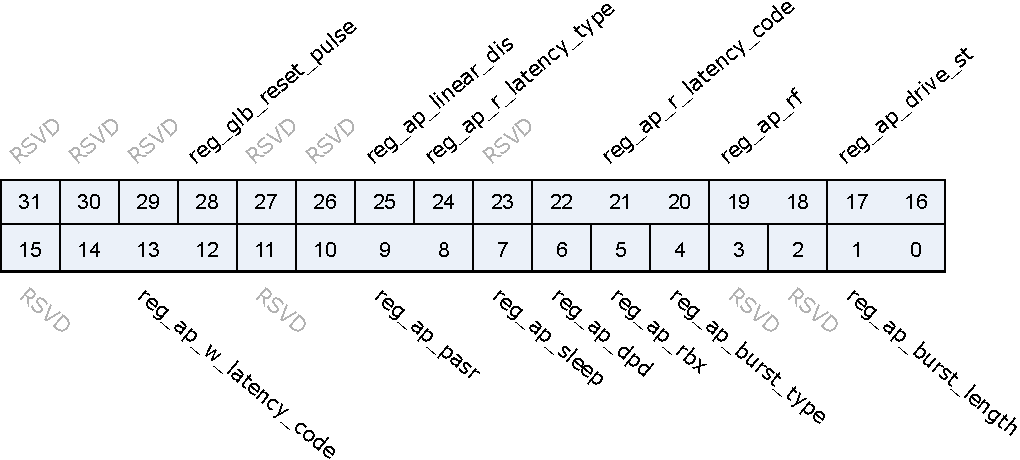
\includegraphics{psram_apmemory_psram_configure.pdf}
\end{figure}

\regdes{31:29&RSVD& & & \\\hline
28&reg\_glb\_reset\_pulse&w1p&1'b0&AP Memory pSRAM global reset enable\\\hline
27:26&RSVD& & & \\\hline
25&reg\_ap\_linear\_dis&r/w&1'b0&AP Memory pSRAM linear burst disable\\\hline
24&reg\_ap\_r\_latency\_type&r/w&1'b0&AP Memory pSRAM configure MR0 - read latency type \par 1'b0 - Variable \par 1'b1 - Fixed
\\\hline
23&RSVD& & & \\\hline
22:20&reg\_ap\_r\_latency\_code&r/w&3'b010&AP Memory pSRAM configure MR0 - read latency code
 \par 3'b000 - Latency = 3 / Max freq. = 66MHz
 \par 3'b001 - Latency = 4 / Max freq. = 104MHz
 \par 3'b010 - Latency = 5 / Max freq. = 133MHz
 \par 3'b011 - Latency = 6 / Max freq. = 166MHz
 \par 3'b100 - Latency = 7 / Max freq. = 200MHz
 \par Others - RSVD
\\\hline
19:18&reg\_ap\_rf&r/w&1'b0&AP Memory pSRAM configure MR4 - refresh frequency\\\hline
17:16&reg\_ap\_drive\_st&r/w&2'b01&AP Memory pSRAM configure MR0 - drive strength \par 2'b00 - Full (25Ω) \par 2'b01 - Half (50Ω) \par 2'b10 - 1/4 (100Ω) \par 2'b11 - 1/8 (200Ω)
\\\hline
15&RSVD& & & \\\hline
14:12&reg\_ap\_w\_latency\_code&r/w&3'b010&AP Memory pSRAM configure MR4 - write latency code
 \par 3'b000 - Latency = 3 / Max freq. = 66MHz
 \par 3'b100 - Latency = 4 / Max freq. = 104MHz
 \par 3'b010 - Latency = 5 / Max freq. = 133MHz
 \par 3'b110 - Latency = 6 / Max freq. = 166MHz
 \par 3'b001 - Latency = 7 / Max freq. = 200MHz
 \par Others - RSVD
\\\hline
11&RSVD& & & \\\hline
10:8&reg\_ap\_pasr&r/w&3'b000&AP Memory pSRAM configure MR4 - partial array refresh \par 3'b000 - Full array \par 3'b001 - Bottom 1/2 array \par 3'b010 - Bottom 1/4 array \par 3'b011 - Bottom 1/8 array \par 3'b100 - RSVD \par 3'b101 - Top 1/2 array \par 3'b110 - Top 1/4 array \par 3'b111 - Top 1/8 array
\\\hline
7&reg\_ap\_sleep&r/w&1'b0&AP Memory pSRAM configure MR6 - Half Sleep enable\\\hline
6&reg\_ap\_dpd&r/w&1'b0&AP Memory pSRAM configure MR6 - Deep Power Down enable\\\hline
5&reg\_ap\_rbx&r/w&1'b0&AP Memory pSRAM configure MR8 - cross boundary enable \par 1'b0 - Read within 1K boundary \par 1'b1 - Read cross 1K boundary
\\\hline
4&reg\_ap\_burst\_type&r/w&1'b1&AP Memory pSRAM configure MR8 - burst type \par 1'b0 - Normal Wrap \par 1'b1 - Hybrid Wrap
\\\hline
3:2&RSVD& & & \\\hline
1:0&reg\_ap\_burst\_length&r/w&2'b01&AP Memory pSRAM configure MR8 - burst length \par For APS6408L‐OBx \par 2'd0 - 16 Byte \par 2'd1 - 32 Byte \par 2'd2 - 64 Byte \par 2'd3 - 1K  Byte \par For APS256XXN-OBRx \par 2'd0 - 16 Beat \par 2'd1 - 32 Beat \par 2'd2 - 64 Beat \par 2'd3 - 2K  Byte
\\\hline

}
\subsection{apmemory\_psram\_status}
\label{psram-apmemory-psram-status}
地址:0x4001a024
 \begin{figure}[H]
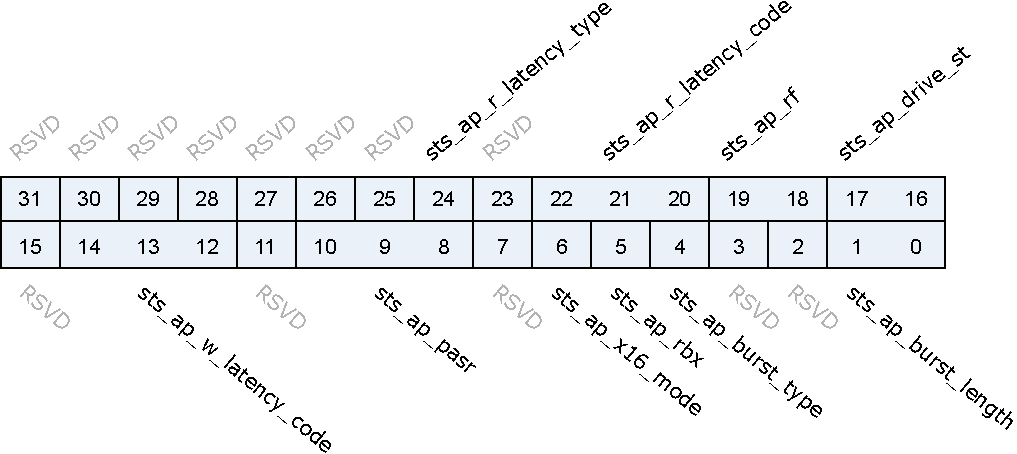
\includegraphics{psram_apmemory_psram_status.pdf}
\end{figure}

\regdes{31:25&RSVD& & & \\\hline
24&sts\_ap\_r\_latency\_type&r&1'b0&AP Memory pSRAM status MR0 - read latency type
 \par 1'b0 - Variable
 \par 1'b1 - Fixed
\\\hline
23&RSVD& & & \\\hline
22:20&sts\_ap\_r\_latency\_code&r&3'b010&AP Memory pSRAM status MR0 - read latency code
 \par 3'b000 - Latency = 3 / Mas freq. = 66MHz
 \par 3'b001 - Latency = 4 / Mas freq. = 104MHz
 \par 3'b010 - Latency = 5 / Mas freq. = 133MHz
 \par 3'b011 - Latency = 6 / Mas freq. = 166MHz
 \par 3'b100 - Latency = 7 / Mas freq. = 200MHz
 \par Others - RSVD
\\\hline
19:18&sts\_ap\_rf&r&1'b0&AP Memory pSRAM configure MR4 - refresh frequency\\\hline
17:16&sts\_ap\_drive\_st&r&2'b01&AP Memory pSRAM status MR0 - drive strength
 \par 2'b00 - Full (25Ω)
 \par 2'b01 - Half (50Ω)
 \par 2'b10 - 1/4 (100Ω)
 \par 2'b11 - 1/8 (200Ω)
\\\hline
15&RSVD& & & \\\hline
14:12&sts\_ap\_w\_latency\_code&r&3'b010&AP Memory pSRAM status MR4 - write latency code
 \par 3'b000 - Latency = 3 / Mas freq. = 66MHz
 \par 3'b100 - Latency = 4 / Mas freq. = 104MHz
 \par 3'b010 - Latency = 5 / Mas freq. = 133MHz
 \par 3'b110 - Latency = 6 / Mas freq. = 166MHz
 \par 3'b001 - Latency = 7 / Mas freq. = 200MHz
 \par Others - RSVD
\\\hline
11&RSVD& & & \\\hline
10:8&sts\_ap\_pasr&r&3'b000&AP Memory pSRAM status MR4 - partial array refresh
 \par 3'b000 - Full array
 \par 3'b001 - Bottom 1/2 array
 \par 3'b010 - Bottom 1/4 array
 \par 3'b011 - Bottom 1/8 array
 \par 3'b100 - RSVD
 \par 3'b101 - Top 1/2 array
 \par 3'b110 - Top 1/4 array
 \par 3'b111 - Top 1/8 array
\\\hline
7&RSVD& & & \\\hline
6&sts\_ap\_x16\_mode&r&1'b0&AP Memory pSRAM status MR8 - X16 mode enable\\\hline
5&sts\_ap\_rbx&r&1'b0&AP Memory pSRAM status MR8 - cross boundary enable
 \par 1'b0 - Read within 1K boundary
 \par 1'b1 - Read cross 1K boundary
\\\hline
4&sts\_ap\_burst\_type&r&1'b1&AP Memory pSRAM status MR8 - burst type
 \par 1'b0 - Normal Wrap
 \par 1'b1 - Hybrid Wrap
\\\hline
3:2&RSVD& & & \\\hline
1:0&sts\_ap\_burst\_length&r&2'b01&AP Memory pSRAM configure MR8 - burst length \par For APS6408L‐OBx \par 2'd0 - 16 Byte \par 2'd1 - 32 Byte \par 2'd2 - 64 Byte \par 2'd3 - 1K  Byte \par For APS256XXN-OBRx \par 2'd0 - 16 Beat \par 2'd1 - 32 Beat \par 2'd2 - 64 Beat \par 2'd3 - 2K  Byte
\\\hline

}
\subsection{psram\_manual\_control3}
\label{psram-psram-manual-control3}
地址:0x4001a030
 \begin{figure}[H]
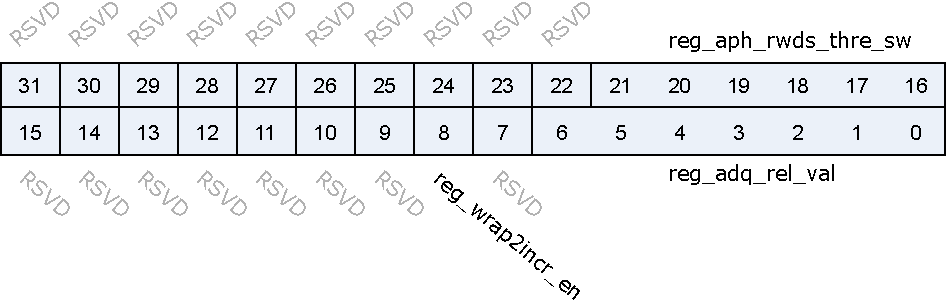
\includegraphics{psram_psram_manual_control3.pdf}
\end{figure}

\regdes{31:22&RSVD& & & \\\hline
21:16&reg\_aph\_rwds\_thre\_sw&r/w&6'h0&APH RWDS threshold in sw mode (reg\_wc\_sw\_en=1)\\\hline
15:9&RSVD& & & \\\hline
8&reg\_wrap2incr\_en&r/w&1'b1&Auto wrap to increament enable\\\hline
7&RSVD& & & \\\hline
6:0&reg\_adq\_rel\_val&r/w&7'h20&pSRAM adq\_oen release counter value\\\hline

}
\subsection{psram\_intf\_delay\_ctrl0}
\label{psram-psram-intf-delay-ctrl0}
地址:0x4001a080
 \begin{figure}[H]
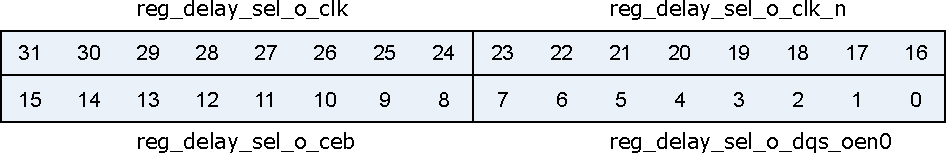
\includegraphics{psram_psram_intf_delay_ctrl0.pdf}
\end{figure}

\regdes{31:24&reg\_delay\_sel\_o\_clk&r/w&8'h0&Output Delay Chain Control - clk\\\hline
23:16&reg\_delay\_sel\_o\_clk\_n&r/w&8'h0&Output Delay Chain Control - clk\_n\\\hline
15:8&reg\_delay\_sel\_o\_ceb&r/w&8'h0&Output Delay Chain Control - ceb\\\hline
7:0&reg\_delay\_sel\_o\_dqs\_oen0&r/w&8'h0&Output Delay Chain Control - dqs\_oen[0]\\\hline

}
\subsection{psram\_intf\_delay\_ctrl1}
\label{psram-psram-intf-delay-ctrl1}
地址:0x4001a084
 \begin{figure}[H]
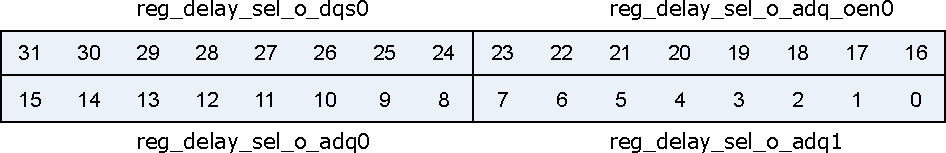
\includegraphics{psram_psram_intf_delay_ctrl1.pdf}
\end{figure}

\regdes{31:24&reg\_delay\_sel\_o\_dqs0&r/w&8'h0&Output Delay Chain Control - dqs\_o[0]\\\hline
23:16&reg\_delay\_sel\_o\_adq\_oen0&r/w&8'h0&Output Delay Chain Control - adq\_oen[0]\\\hline
15:8&reg\_delay\_sel\_o\_adq0&r/w&8'h0&Output Delay Chain Control - adq\_o[0]\\\hline
7:0&reg\_delay\_sel\_o\_adq1&r/w&8'h0&Output Delay Chain Control - adq\_o[1]\\\hline

}
\subsection{psram\_intf\_delay\_ctrl2}
\label{psram-psram-intf-delay-ctrl2}
地址:0x4001a088
 \begin{figure}[H]
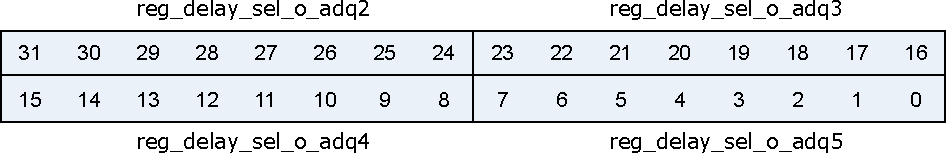
\includegraphics{psram_psram_intf_delay_ctrl2.pdf}
\end{figure}

\regdes{31:24&reg\_delay\_sel\_o\_adq2&r/w&8'h0&Output Delay Chain Control - adq\_o[2]\\\hline
23:16&reg\_delay\_sel\_o\_adq3&r/w&8'h0&Output Delay Chain Control - adq\_o[3]\\\hline
15:8&reg\_delay\_sel\_o\_adq4&r/w&8'h0&Output Delay Chain Control - adq\_o[4]\\\hline
7:0&reg\_delay\_sel\_o\_adq5&r/w&8'h0&Output Delay Chain Control - adq\_o[5]\\\hline

}
\subsection{psram\_intf\_delay\_ctrl3}
\label{psram-psram-intf-delay-ctrl3}
地址:0x4001a08c
 \begin{figure}[H]
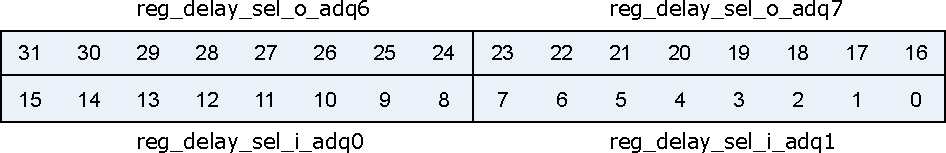
\includegraphics{psram_psram_intf_delay_ctrl3.pdf}
\end{figure}

\regdes{31:24&reg\_delay\_sel\_o\_adq6&r/w&8'h0&Output Delay Chain Control - adq\_o[6]\\\hline
23:16&reg\_delay\_sel\_o\_adq7&r/w&8'h0&Output Delay Chain Control - adq\_o[7]\\\hline
15:8&reg\_delay\_sel\_i\_adq0&r/w&8'h0&Input Delay Chain Control - adq\_i[0]\\\hline
7:0&reg\_delay\_sel\_i\_adq1&r/w&8'h0&Input Delay Chain Control - adq\_i[1]\\\hline

}
\subsection{psram\_intf\_delay\_ctrl4}
\label{psram-psram-intf-delay-ctrl4}
地址:0x4001a090
 \begin{figure}[H]
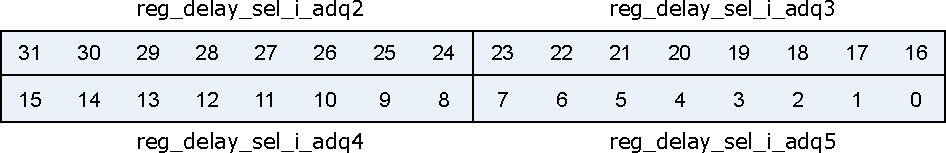
\includegraphics{psram_psram_intf_delay_ctrl4.pdf}
\end{figure}

\regdes{31:24&reg\_delay\_sel\_i\_adq2&r/w&8'h0&Input Delay Chain Control - adq\_i[2]\\\hline
23:16&reg\_delay\_sel\_i\_adq3&r/w&8'h0&Input Delay Chain Control - adq\_i[3]\\\hline
15:8&reg\_delay\_sel\_i\_adq4&r/w&8'h0&Input Delay Chain Control - adq\_i[4]\\\hline
7:0&reg\_delay\_sel\_i\_adq5&r/w&8'h0&Input Delay Chain Control - adq\_i[5]\\\hline

}
\subsection{psram\_intf\_delay\_ctrl5}
\label{psram-psram-intf-delay-ctrl5}
地址:0x4001a094
 \begin{figure}[H]
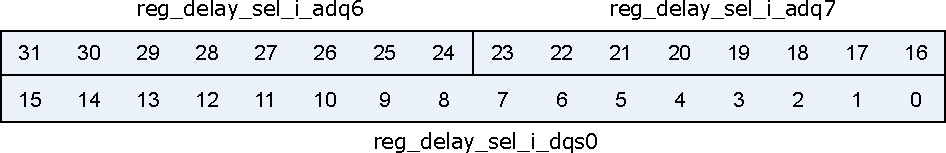
\includegraphics{psram_psram_intf_delay_ctrl5.pdf}
\end{figure}

\regdes{31:24&reg\_delay\_sel\_i\_adq6&r/w&8'h0&Input Delay Chain Control - adq\_i[6]\\\hline
23:16&reg\_delay\_sel\_i\_adq7&r/w&8'h0&Input Delay Chain Control - adq\_i[7]\\\hline
15:0&reg\_delay\_sel\_i\_dqs0&r/w&16'h0&Input Delay Chain Control - dqs\_i[0]\\\hline

}
\subsection{psram\_intf\_delay\_ctrl6}
\label{psram-psram-intf-delay-ctrl6}
地址:0x4001a098
 \begin{figure}[H]
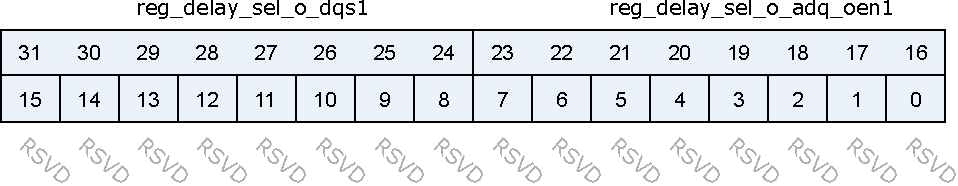
\includegraphics{psram_psram_intf_delay_ctrl6.pdf}
\end{figure}

\regdes{31:24&reg\_delay\_sel\_o\_dqs1&r/w&8'h0&Output Delay Chain Control - dqs\_o[1]\\\hline
23:16&reg\_delay\_sel\_o\_adq\_oen1&r/w&8'h0&Output Delay Chain Control - adq\_oen[1]\\\hline
15:0&RSVD& & & \\\hline

}
\subsection{psram\_intf\_delay\_ctrlB}
\label{psram-psram-intf-delay-ctrlB}
地址:0x4001a0ac
 \begin{figure}[H]
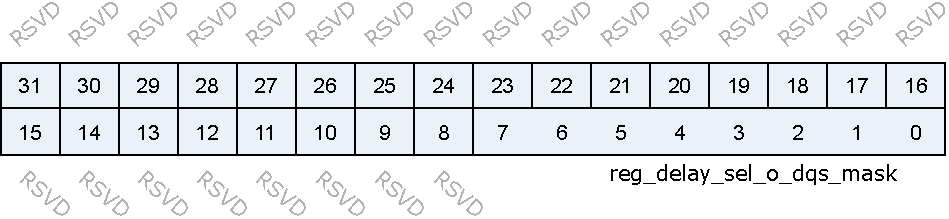
\includegraphics{psram_psram_intf_delay_ctrlB.pdf}
\end{figure}

\regdes{31:8&RSVD& & & \\\hline
7:0&reg\_delay\_sel\_o\_dqs\_mask&r/w&8'h0&Output Delay Chain Control - adq\_mask\\\hline

}
\subsection{psram\_dbg\_sel}
\label{psram-psram-dbg-sel}
地址:0x4001a0c0
 \begin{figure}[H]
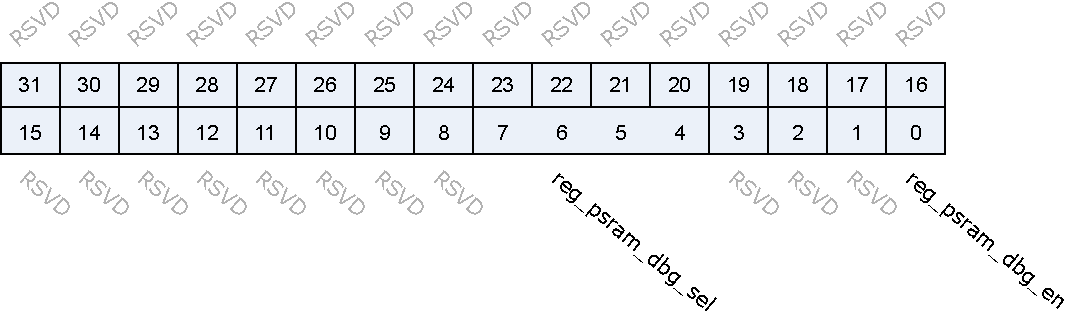
\includegraphics{psram_psram_dbg_sel.pdf}
\end{figure}

\regdes{31:8&RSVD& & & \\\hline
7:4&reg\_psram\_dbg\_sel&r/w&4'd0&pSRAM debug selection\\\hline
3:1&RSVD& & & \\\hline
0&reg\_psram\_dbg\_en&r/w&1'b0&pSRAM debug enable\\\hline

}
\subsection{psram\_dummy\_reg}
\label{psram-psram-dummy-reg}
地址:0x4001a0f0
 \begin{figure}[H]
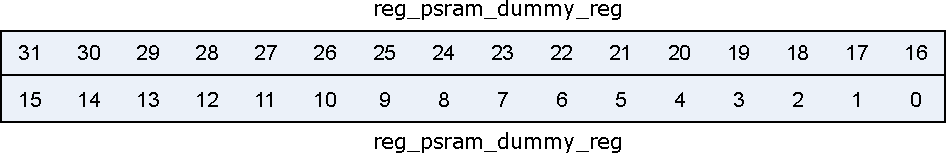
\includegraphics{psram_psram_dummy_reg.pdf}
\end{figure}

\regdes{31:0&reg\_psram\_dummy\_reg&r/w&32'hFFFF0000&pSRAM Dummy register\\\hline

}
\subsection{psram\_timeout\_reg}
\label{psram-psram-timeout-reg}
地址:0x4001a0f4
 \begin{figure}[H]
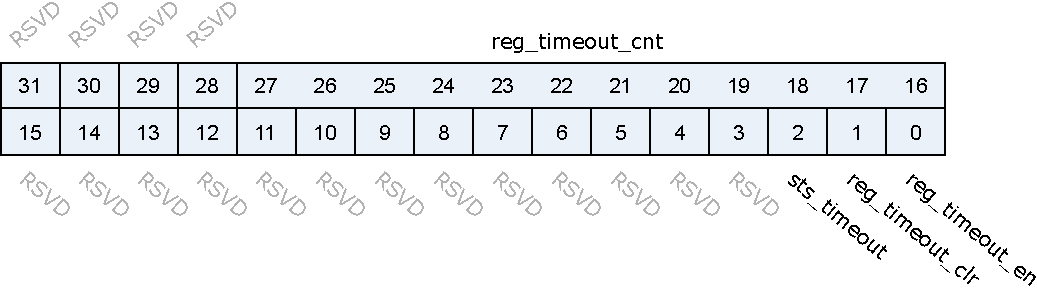
\includegraphics{psram_psram_timeout_reg.pdf}
\end{figure}

\regdes{31:28&RSVD& & & \\\hline
27:16&reg\_timeout\_cnt&r/w&12'h100&Timeout threshold\\\hline
15:3&RSVD& & & \\\hline
2&sts\_timeout&r&1'h0&Timeout status\\\hline
1&reg\_timeout\_clr&r/w&1'h0&Timeout status clear\\\hline
0&reg\_timeout\_en&r/w&1'h0&Timeout enable\\\hline

}
\subsection{psram\_rough\_delay\_ctrl0}
\label{psram-psram-rough-delay-ctrl0}
地址:0x4001a100
 \begin{figure}[H]
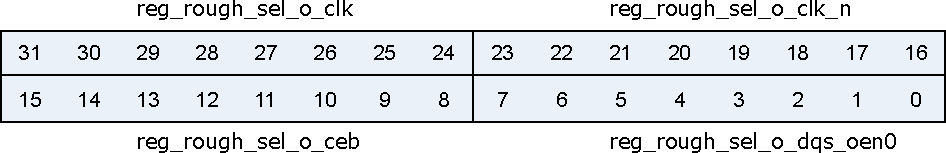
\includegraphics{psram_psram_rough_delay_ctrl0.pdf}
\end{figure}

\regdes{31:24&reg\_rough\_sel\_o\_clk&r/w&8'h0&Output Delay Chain Control - clk\\\hline
23:16&reg\_rough\_sel\_o\_clk\_n&r/w&8'h0&Output Delay Chain Control - clk\_n\\\hline
15:8&reg\_rough\_sel\_o\_ceb&r/w&8'h0&Output Delay Chain Control - ceb\\\hline
7:0&reg\_rough\_sel\_o\_dqs\_oen0&r/w&8'h0&Output Delay Chain Control - dqs\_oen[0]\\\hline

}
\subsection{psram\_rough\_delay\_ctrl1}
\label{psram-psram-rough-delay-ctrl1}
地址:0x4001a104
 \begin{figure}[H]
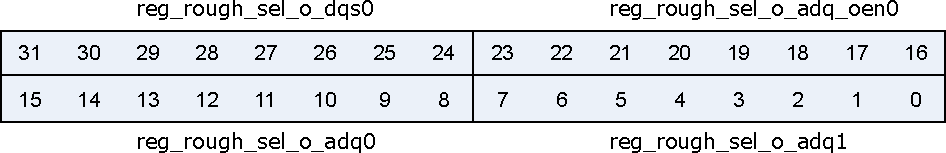
\includegraphics{psram_psram_rough_delay_ctrl1.pdf}
\end{figure}

\regdes{31:24&reg\_rough\_sel\_o\_dqs0&r/w&8'h0&Output Delay Chain Control - dqs\_o[0]\\\hline
23:16&reg\_rough\_sel\_o\_adq\_oen0&r/w&8'h0&Output Delay Chain Control - adq\_oen[0]\\\hline
15:8&reg\_rough\_sel\_o\_adq0&r/w&8'h0&Output Delay Chain Control - adq\_o[0]\\\hline
7:0&reg\_rough\_sel\_o\_adq1&r/w&8'h0&Output Delay Chain Control - adq\_o[1]\\\hline

}
\subsection{psram\_rough\_delay\_ctrl2}
\label{psram-psram-rough-delay-ctrl2}
地址:0x4001a108
 \begin{figure}[H]
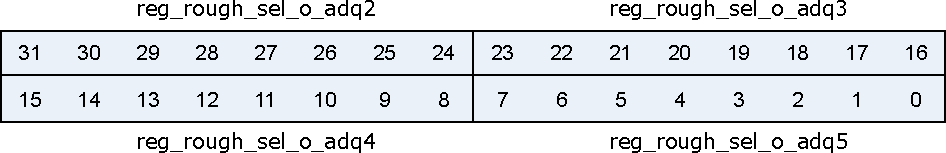
\includegraphics{psram_psram_rough_delay_ctrl2.pdf}
\end{figure}

\regdes{31:24&reg\_rough\_sel\_o\_adq2&r/w&8'h0&Output Delay Chain Control - adq\_o[2]\\\hline
23:16&reg\_rough\_sel\_o\_adq3&r/w&8'h0&Output Delay Chain Control - adq\_o[3]\\\hline
15:8&reg\_rough\_sel\_o\_adq4&r/w&8'h0&Output Delay Chain Control - adq\_o[4]\\\hline
7:0&reg\_rough\_sel\_o\_adq5&r/w&8'h0&Output Delay Chain Control - adq\_o[5]\\\hline

}
\subsection{psram\_rough\_delay\_ctrl3}
\label{psram-psram-rough-delay-ctrl3}
地址:0x4001a10c
 \begin{figure}[H]
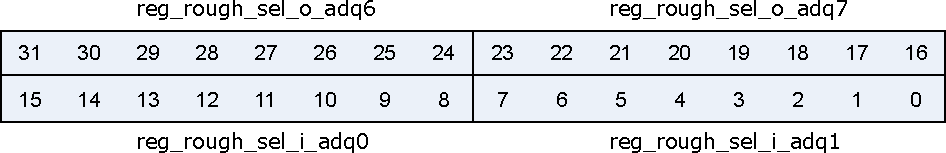
\includegraphics{psram_psram_rough_delay_ctrl3.pdf}
\end{figure}

\regdes{31:24&reg\_rough\_sel\_o\_adq6&r/w&8'h0&Output Delay Chain Control - adq\_o[6]\\\hline
23:16&reg\_rough\_sel\_o\_adq7&r/w&8'h0&Output Delay Chain Control - adq\_o[7]\\\hline
15:8&reg\_rough\_sel\_i\_adq0&r/w&8'h0&Input Delay Chain Control - adq\_i[0]\\\hline
7:0&reg\_rough\_sel\_i\_adq1&r/w&8'h0&Input Delay Chain Control - adq\_i[1]\\\hline

}
\subsection{psram\_rough\_delay\_ctrl4}
\label{psram-psram-rough-delay-ctrl4}
地址:0x4001a110
 \begin{figure}[H]
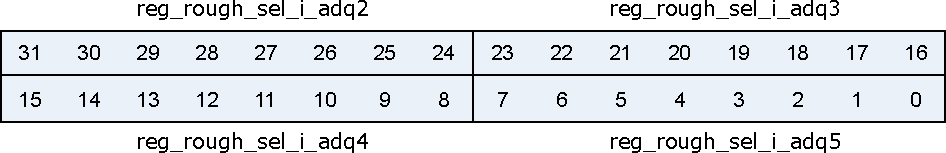
\includegraphics{psram_psram_rough_delay_ctrl4.pdf}
\end{figure}

\regdes{31:24&reg\_rough\_sel\_i\_adq2&r/w&8'h0&Input Delay Chain Control - adq\_i[2]\\\hline
23:16&reg\_rough\_sel\_i\_adq3&r/w&8'h0&Input Delay Chain Control - adq\_i[3]\\\hline
15:8&reg\_rough\_sel\_i\_adq4&r/w&8'h0&Input Delay Chain Control - adq\_i[4]\\\hline
7:0&reg\_rough\_sel\_i\_adq5&r/w&8'h0&Input Delay Chain Control - adq\_i[5]\\\hline

}
\subsection{psram\_rough\_delay\_ctrl5}
\label{psram-psram-rough-delay-ctrl5}
地址:0x4001a114
 \begin{figure}[H]
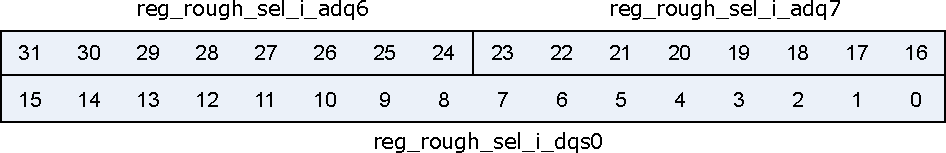
\includegraphics{psram_psram_rough_delay_ctrl5.pdf}
\end{figure}

\regdes{31:24&reg\_rough\_sel\_i\_adq6&r/w&8'h0&Input Delay Chain Control - adq\_i[6]\\\hline
23:16&reg\_rough\_sel\_i\_adq7&r/w&8'h0&Input Delay Chain Control - adq\_i[7]\\\hline
15:0&reg\_rough\_sel\_i\_dqs0&r/w&16'h0&Input Delay Chain Control - dqs\_i[0]\\\hline

}
\subsection{psram\_rough\_delay\_ctrl6}
\label{psram-psram-rough-delay-ctrl6}
地址:0x4001a118
 \begin{figure}[H]
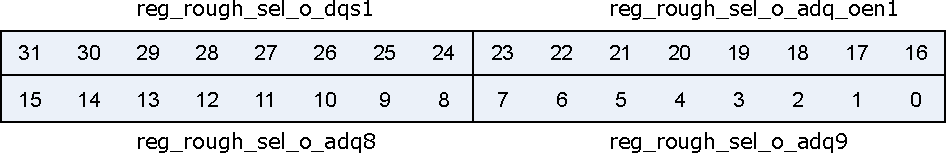
\includegraphics{psram_psram_rough_delay_ctrl6.pdf}
\end{figure}

\regdes{31:24&reg\_rough\_sel\_o\_dqs1&r/w&8'h0&Output Delay Chain Control - dqs\_o[1]\\\hline
23:16&reg\_rough\_sel\_o\_adq\_oen1&r/w&8'h0&Output Delay Chain Control - adq\_oen[1]\\\hline
15:8&reg\_rough\_sel\_o\_adq8&r/w&8'h0&Output Delay Chain Control - adq\_o[8]\\\hline
7:0&reg\_rough\_sel\_o\_adq9&r/w&8'h0&Output Delay Chain Control - adq\_o[9]\\\hline

}
\subsection{psram\_rough\_delay\_ctrl7}
\label{psram-psram-rough-delay-ctrl7}
地址:0x4001a11c
 \begin{figure}[H]
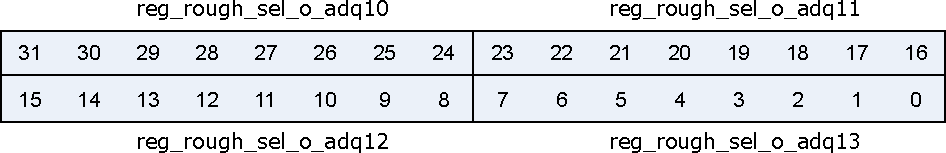
\includegraphics{psram_psram_rough_delay_ctrl7.pdf}
\end{figure}

\regdes{31:24&reg\_rough\_sel\_o\_adq10&r/w&8'h0&Output Delay Chain Control - adq\_o[10]\\\hline
23:16&reg\_rough\_sel\_o\_adq11&r/w&8'h0&Output Delay Chain Control - adq\_o[11]\\\hline
15:8&reg\_rough\_sel\_o\_adq12&r/w&8'h0&Output Delay Chain Control - adq\_o[12]\\\hline
7:0&reg\_rough\_sel\_o\_adq13&r/w&8'h0&Output Delay Chain Control - adq\_o[13]\\\hline

}
\subsection{psram\_rough\_delay\_ctrl8}
\label{psram-psram-rough-delay-ctrl8}
地址:0x4001a120
 \begin{figure}[H]
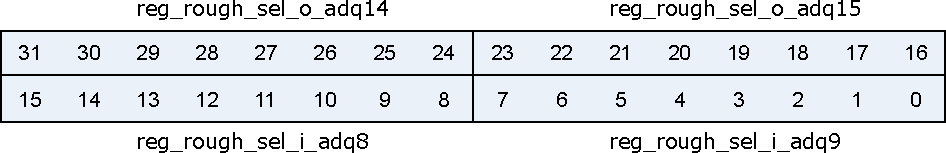
\includegraphics{psram_psram_rough_delay_ctrl8.pdf}
\end{figure}

\regdes{31:24&reg\_rough\_sel\_o\_adq14&r/w&8'h0&Output Delay Chain Control - adq\_o[14]\\\hline
23:16&reg\_rough\_sel\_o\_adq15&r/w&8'h0&Output Delay Chain Control - adq\_o[15]\\\hline
15:8&reg\_rough\_sel\_i\_adq8&r/w&8'h0&Input Delay Chain Control - adq\_i[8]\\\hline
7:0&reg\_rough\_sel\_i\_adq9&r/w&8'h0&Input Delay Chain Control - adq\_i[9]\\\hline

}
\subsection{psram\_rough\_delay\_ctrl9}
\label{psram-psram-rough-delay-ctrl9}
地址:0x4001a124
 \begin{figure}[H]
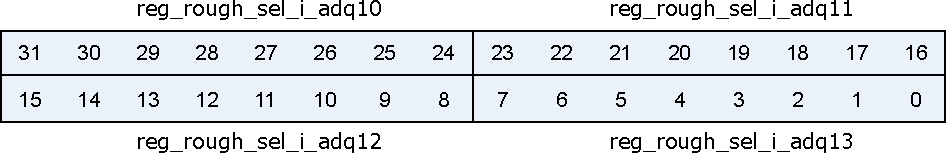
\includegraphics{psram_psram_rough_delay_ctrl9.pdf}
\end{figure}

\regdes{31:24&reg\_rough\_sel\_i\_adq10&r/w&8'h0&Input Delay Chain Control - adq\_i[10]\\\hline
23:16&reg\_rough\_sel\_i\_adq11&r/w&8'h0&Input Delay Chain Control - adq\_i[11]\\\hline
15:8&reg\_rough\_sel\_i\_adq12&r/w&8'h0&Input Delay Chain Control - adq\_i[12]\\\hline
7:0&reg\_rough\_sel\_i\_adq13&r/w&8'h0&Input Delay Chain Control - adq\_i[13]\\\hline

}
\subsection{psram\_rough\_delay\_ctrlA}
\label{psram-psram-rough-delay-ctrlA}
地址:0x4001a128
 \begin{figure}[H]
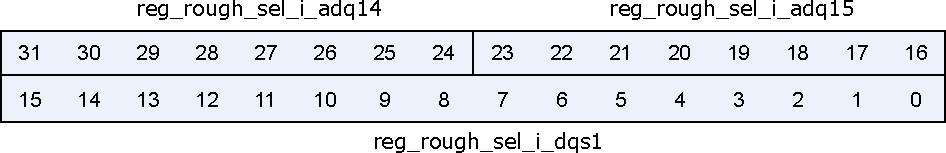
\includegraphics{psram_psram_rough_delay_ctrlA.pdf}
\end{figure}

\regdes{31:24&reg\_rough\_sel\_i\_adq14&r/w&8'h0&Input Delay Chain Control - adq\_i[14]\\\hline
23:16&reg\_rough\_sel\_i\_adq15&r/w&8'h0&Input Delay Chain Control - adq\_i[15]\\\hline
15:0&reg\_rough\_sel\_i\_dqs1&r/w&16'h0&Input Delay Chain Control - dqs\_i[1]\\\hline

}
\subsection{psram\_rough\_delay\_ctrlB}
\label{psram-psram-rough-delay-ctrlB}
地址:0x4001a12c
 \begin{figure}[H]
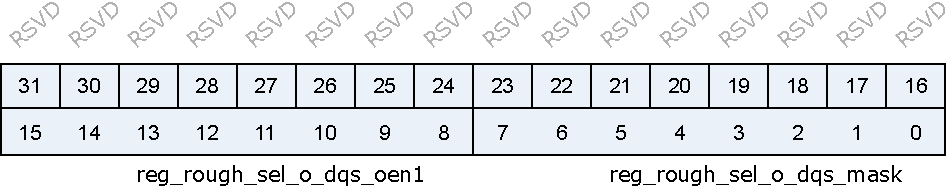
\includegraphics{psram_psram_rough_delay_ctrlB.pdf}
\end{figure}

\regdes{31:16&RSVD& & & \\\hline
15:8&reg\_rough\_sel\_o\_dqs\_oen1&r/w&8'h0&Output Delay Chain Control - dqs\_oen[1]\\\hline
7:0&reg\_rough\_sel\_o\_dqs\_mask&r/w&8'h0&Output Delay Chain Control - adq\_mask\\\hline

}
